\section{Numerical illustrations}\label{sec:numerical}
We compare the exact rotating-reaction values with numerical approximations
to finite-dimensional SDP minima on the unit interval, with $n=2$, $d=1$,
and entrywise transport dimension $k=2$. Let $N_t,N_x$ be positive integers
and set $\Delta s=1/N_t$, $\Delta x=1/N_x$.
Mass matrices $M_{k,i}\in\Sp^2$ are sampled at time nodes $k=0,\ldots,N_t$
and cell centres $i=1,\ldots,N_x$. Here $k$ is a local time index.
Full flux matrices $Q_{k,i+1/2}\in\R^{2\times2}$ are sampled at time
midpoints $k=0,\ldots,N_t-1$ and interior faces $i=1,\ldots,N_x-1$;
full reactions $R_{k,i}\in\R^{2\times2}$ use the same time midpoints and
all cells. Exterior fluxes satisfy $Q_{k,1/2}=Q_{k,N_x+1/2}=0$.
For $0\le k<N_t$ and $1\le i\le N_x$, the discrete continuity equation is
\[
 \frac{M_{k+1,i}-M_{k,i}}{\Delta s}
 +\frac{\sym Q_{k,i+1/2}-\sym Q_{k,i-1/2}}{\Delta x}
 =\sym R_{k,i}.
\]
The endpoint matrices are fixed and every nodal mass is PSD.
The mass used in each reaction cost is the arithmetic mean of its two
neighbouring time samples; the face mass additionally averages the two
adjacent cells. For each channel, we impose the $4\times4$ PSD constraint
\[
 \begin{pmatrix}\overline M&Z\\Z^T&S\end{pmatrix}\succeq0,
 \qquad Z=QL^{-1}\ \text{or}\ RH^{-1},\qquad S\in\mathbb S^2,
\]
where $Q$ is the corresponding local flux matrix and each channel has
its own auxiliary matrix $S$.
The objective is $\Delta s\Delta x/2$ times the sum of the auxiliary traces,
with the same factor $1/2$ as \eqref{eq:action}. All weights passed to the
solver are positive definite; the balanced comparison instead sets $R=0$.
We use CVXPY~1.7.2 with Clarabel~0.11.1, absolute and relative gap and
feasibility tolerances $10^{-9}$, and a limit of 300 iterations.
Postprocessing uses a threshold of $10^{-7}$ for absolute and scaled
continuity-equation and endpoint residuals, scaled cone violations,
symmetry errors, boundary fluxes and range residuals; mass eigenvalues
must be at least $-10^{-7}$. The epigraph action and independently
recomputed quadratic action $J_{\rm quad}$ must differ by at most
$10^{-7}+10^{-6}|J_{\rm quad}|$.

Figure~\ref{fig:numerical}(a) evaluates the exact formula in
Proposition~\ref{prop:reactionrotation} along its three reaction regimes
$\theta=\varepsilon^{3/4},\varepsilon^{1/2},\varepsilon^{1/4}$, whose limits
as $\varepsilon\to0$ are $V_*$, $V_*+1/2$ and $+\infty$.
For panel (b), $N_x=1$ and $N_t=8,16,32$; the two reaction weights have
$(\varepsilon,\theta)=(0.4,0.2)$ and $(0.2,0.35)$.
The absolute differences from the continuum formula decrease by about a
factor of four at each temporal refinement, from approximately
$1.65\times10^{-4}$ and $1.69\times10^{-4}$ to
$1.03\times10^{-5}$ and $1.06\times10^{-5}$, respectively.

For panel (c), take $N_x=4$, $N_t=16$, $H=I_2$, $L=tI_2$ and sample
\[
 G_0(x)=I_2+\tfrac14\cos(2\pi x)\diag(1,-1),\qquad
 G_1(x)=I_2+\tfrac14\sin(2\pi x)
                  \begin{pmatrix}0&1\\1&0\end{pmatrix}
\]
at the cell centres. Both continuum total matrices equal $I_2$, so
$E_H=0$. Their traces are identically two, and their hub moments about
$x_*=1/2$ are $2\int_0^1(x-1/2)^2dx=1/6$. Thus
Theorem~\ref{thm:hub} gives the continuum upper bound $1/(3t^2)$.
For $t=1,2,4$, the computed grid values are approximately
$0.003604$, $0.0009564$ and $0.0002429$.
On the same grid with $L=I_2$, reaction weights
$H=\varepsilon I_2$, $\varepsilon=1,1/4,1/16$, give values increasing
from $0.003604$ to $0.003905$, towards the balanced grid value $0.003906$.

All plotted solver outputs pass the recorded feasibility and objective
checks; the largest recorded primal--dual gap is below $4.5\times10^{-10}$.
These checks include solver statuses, residuals and independent
quadratic-cost evaluations. Panels (b) and (c) compare the stated continuum
references with the SDP values on the specified grids.

\begin{figure}[htbp]
\centering
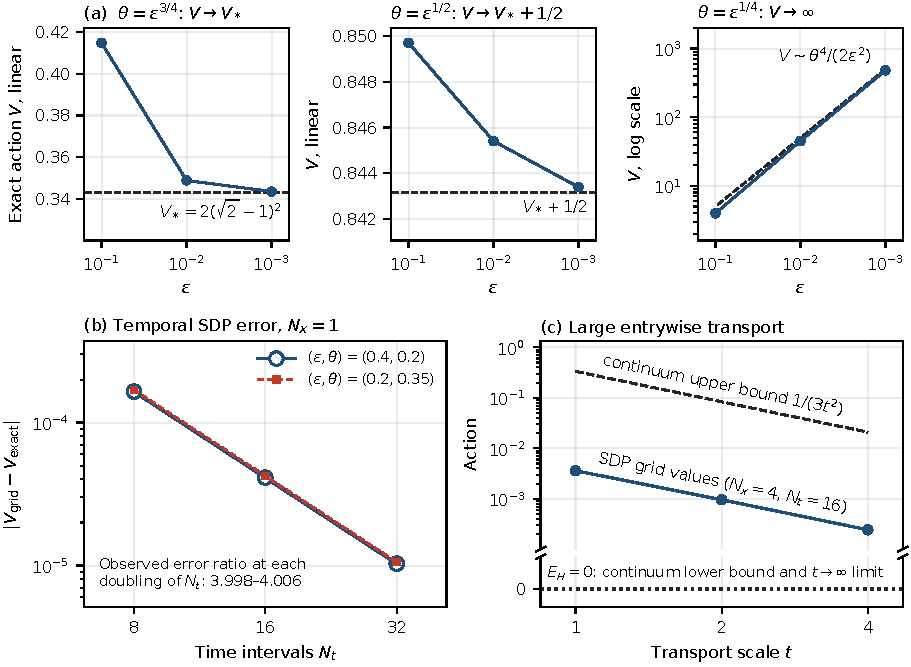
\includegraphics[width=\textwidth]{figures/theory_comparisons.pdf}
\caption{(a) Upper three facets: exact minimum action $V$ of
Proposition~\ref{prop:reactionrotation} for
$\theta=\varepsilon^{3/4},\varepsilon^{1/2},\varepsilon^{1/4}$ at
$\varepsilon=10^{-1},10^{-2},10^{-3}$, on separate vertical axes
(linear, linear, logarithmic). Dashed lines mark the limits
$V_*=2(\sqrt2-1)^2$ and $V_*+1/2$ and the asymptotic reference
$V\sim\theta^4/(2\varepsilon^2)$ of the same proposition.
(b) Absolute differences between SDP values with $N_x=1$ and exact values,
on common axes, for $(\varepsilon,\theta)=(0.4,0.2)$ (circles, solid line)
and $(0.2,0.35)$ (squares, dashed line).
(c) SDP values on the fixed grid $N_x=4$, $N_t=16$ (circles) and the
continuum upper bound $1/(3t^2)$ of Theorem~\ref{thm:hub} (dashed). The
separate linear strip below the axis break marks $E_H=0$ (dotted), the
continuum lower bound and the $t\to\infty$ limit.}
\label{fig:numerical}
\end{figure}
\FloatBarrier
